\documentclass[border={0.1cm 0.1cm 0.1cm 0.1cm}]{standalone}  %E,S,W,N

\usepackage{amssymb}
\usepackage{amsmath}
\usepackage{tikz}

\begin{document}
	
	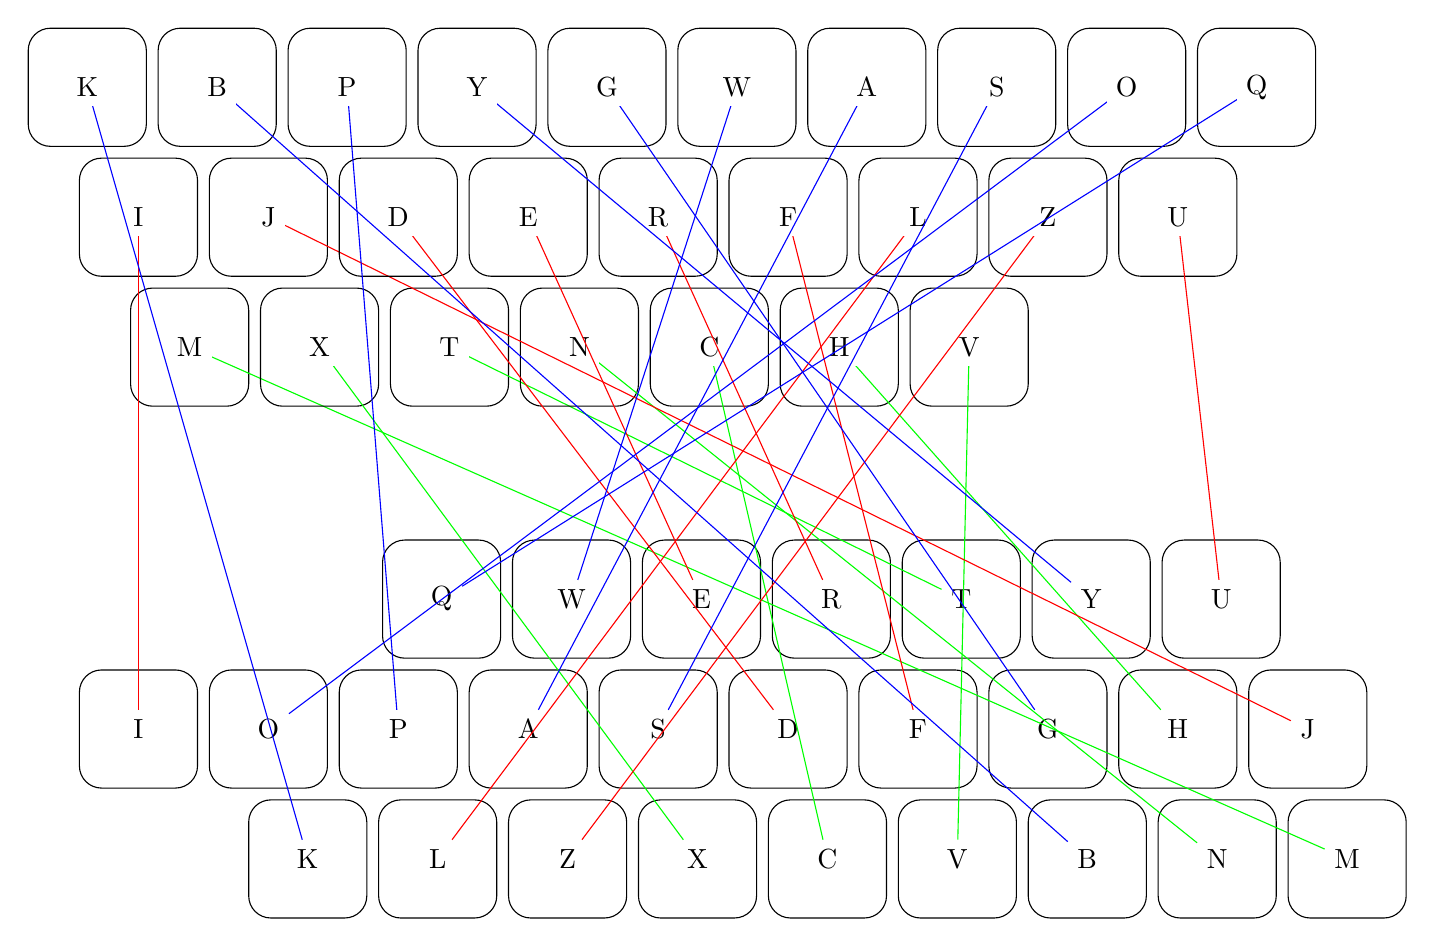
\begin{tikzpicture}	
	\def\s{0.75} %side length for keys
	\def\d{0.15} %distance between keys
	
	%QWERTY
	\foreach \i [count=\j] in {Q,W,E,R,T,Y,U}{ 
		\draw[rounded corners=8pt,yshift=-6.5cm] ({6*\s+(2*\s+\d)*\j-\s},-\s) rectangle ++(2*\s,2*\s);
		\node[yshift=-6.5cm] (\i) at ({6*\s+(2*\s+\d)*\j},0) {\i};
	}
	\foreach \i [count=\j] in {I,O,P,A,S,D,F,G,H,J}{ 
		\draw[rounded corners=8pt,yshift=-6.5cm] ({0.65+(2*\s+\d)*\j-\s},-3*\s-\d) rectangle ++(2*\s,2*\s);
		\node[yshift=-6.5cm] (\i) at ({0.65+(2*\s+\d)*\j},-2*\s-\d) {\i};
	}
	\foreach \i [count=\j] in {K,L,Z,X,C,V,B,N,M}{ 
		\draw[rounded corners=8pt,yshift=-6.5cm] ({2*\s+1.3+(2*\s+\d)*\j-\s},-5*\s-2*\d) rectangle ++(2*\s,2*\s);
		\node[yshift=-6.5cm] (\i) at ({2*\s+1.3+(2*\s+\d)*\j},-4*\s-2*\d) {\i};
	}
	
	%DVORAK-INVERSE
	\foreach \i [count=\j] in {M,X,T,N,C,H,V}{ 
		\draw[rounded corners=8pt] ({1.3+(2*\s+\d)*\j-\s},-5*\s-2*\d) rectangle ++(2*\s,2*\s);
		\draw[green] ({1.3+(2*\s+\d)*\j},-4*\s-2*\d)--(\i);
		\node[fill=white] at ({1.3+(2*\s+\d)*\j},-4*\s-2*\d) {\i};
	}
	\foreach \i [count=\j] in {I,J,D,E,R,F,L,Z,U}{ 
		\draw[rounded corners=8pt] ({0.65+(2*\s+\d)*\j-\s},-3*\s-\d) rectangle ++(2*\s,2*\s);
		\draw[red] ({0.65+(2*\s+\d)*\j},-2*\s-\d)--(\i);
		\node[fill=white] at ({0.65+(2*\s+\d)*\j},-2*\s-\d) {\i};
	}
	\foreach \i [count=\j] in {K,B,P,Y,G,W,A,S,O,Q}{ 
		\draw[rounded corners=8pt] ({(2*\s+\d)*\j-\s},-\s) rectangle ++(2*\s,2*\s);
		\draw[blue] ({(2*\s+\d)*\j},0)--(\i);
		\node[fill=white] at ({(2*\s+\d)*\j},0) {\i};
	}
	\end{tikzpicture}
	
\end{document}